\chapter{Background and Literature Review}\label{chap:litreview}\label{ch:background}

This chapter summarizes the minimum background needed to motivate \textbf{ChromaGuide}: (i) what drives CRISPR-Cas9 on-target efficacy, (ii) how existing predictors model it, and (iii) the key gaps (context and calibrated uncertainty) addressed in this proposal.

\section{CRISPR-Cas9 on-target efficacy: essential biology}

\begin{figure}[htbp]
\centering
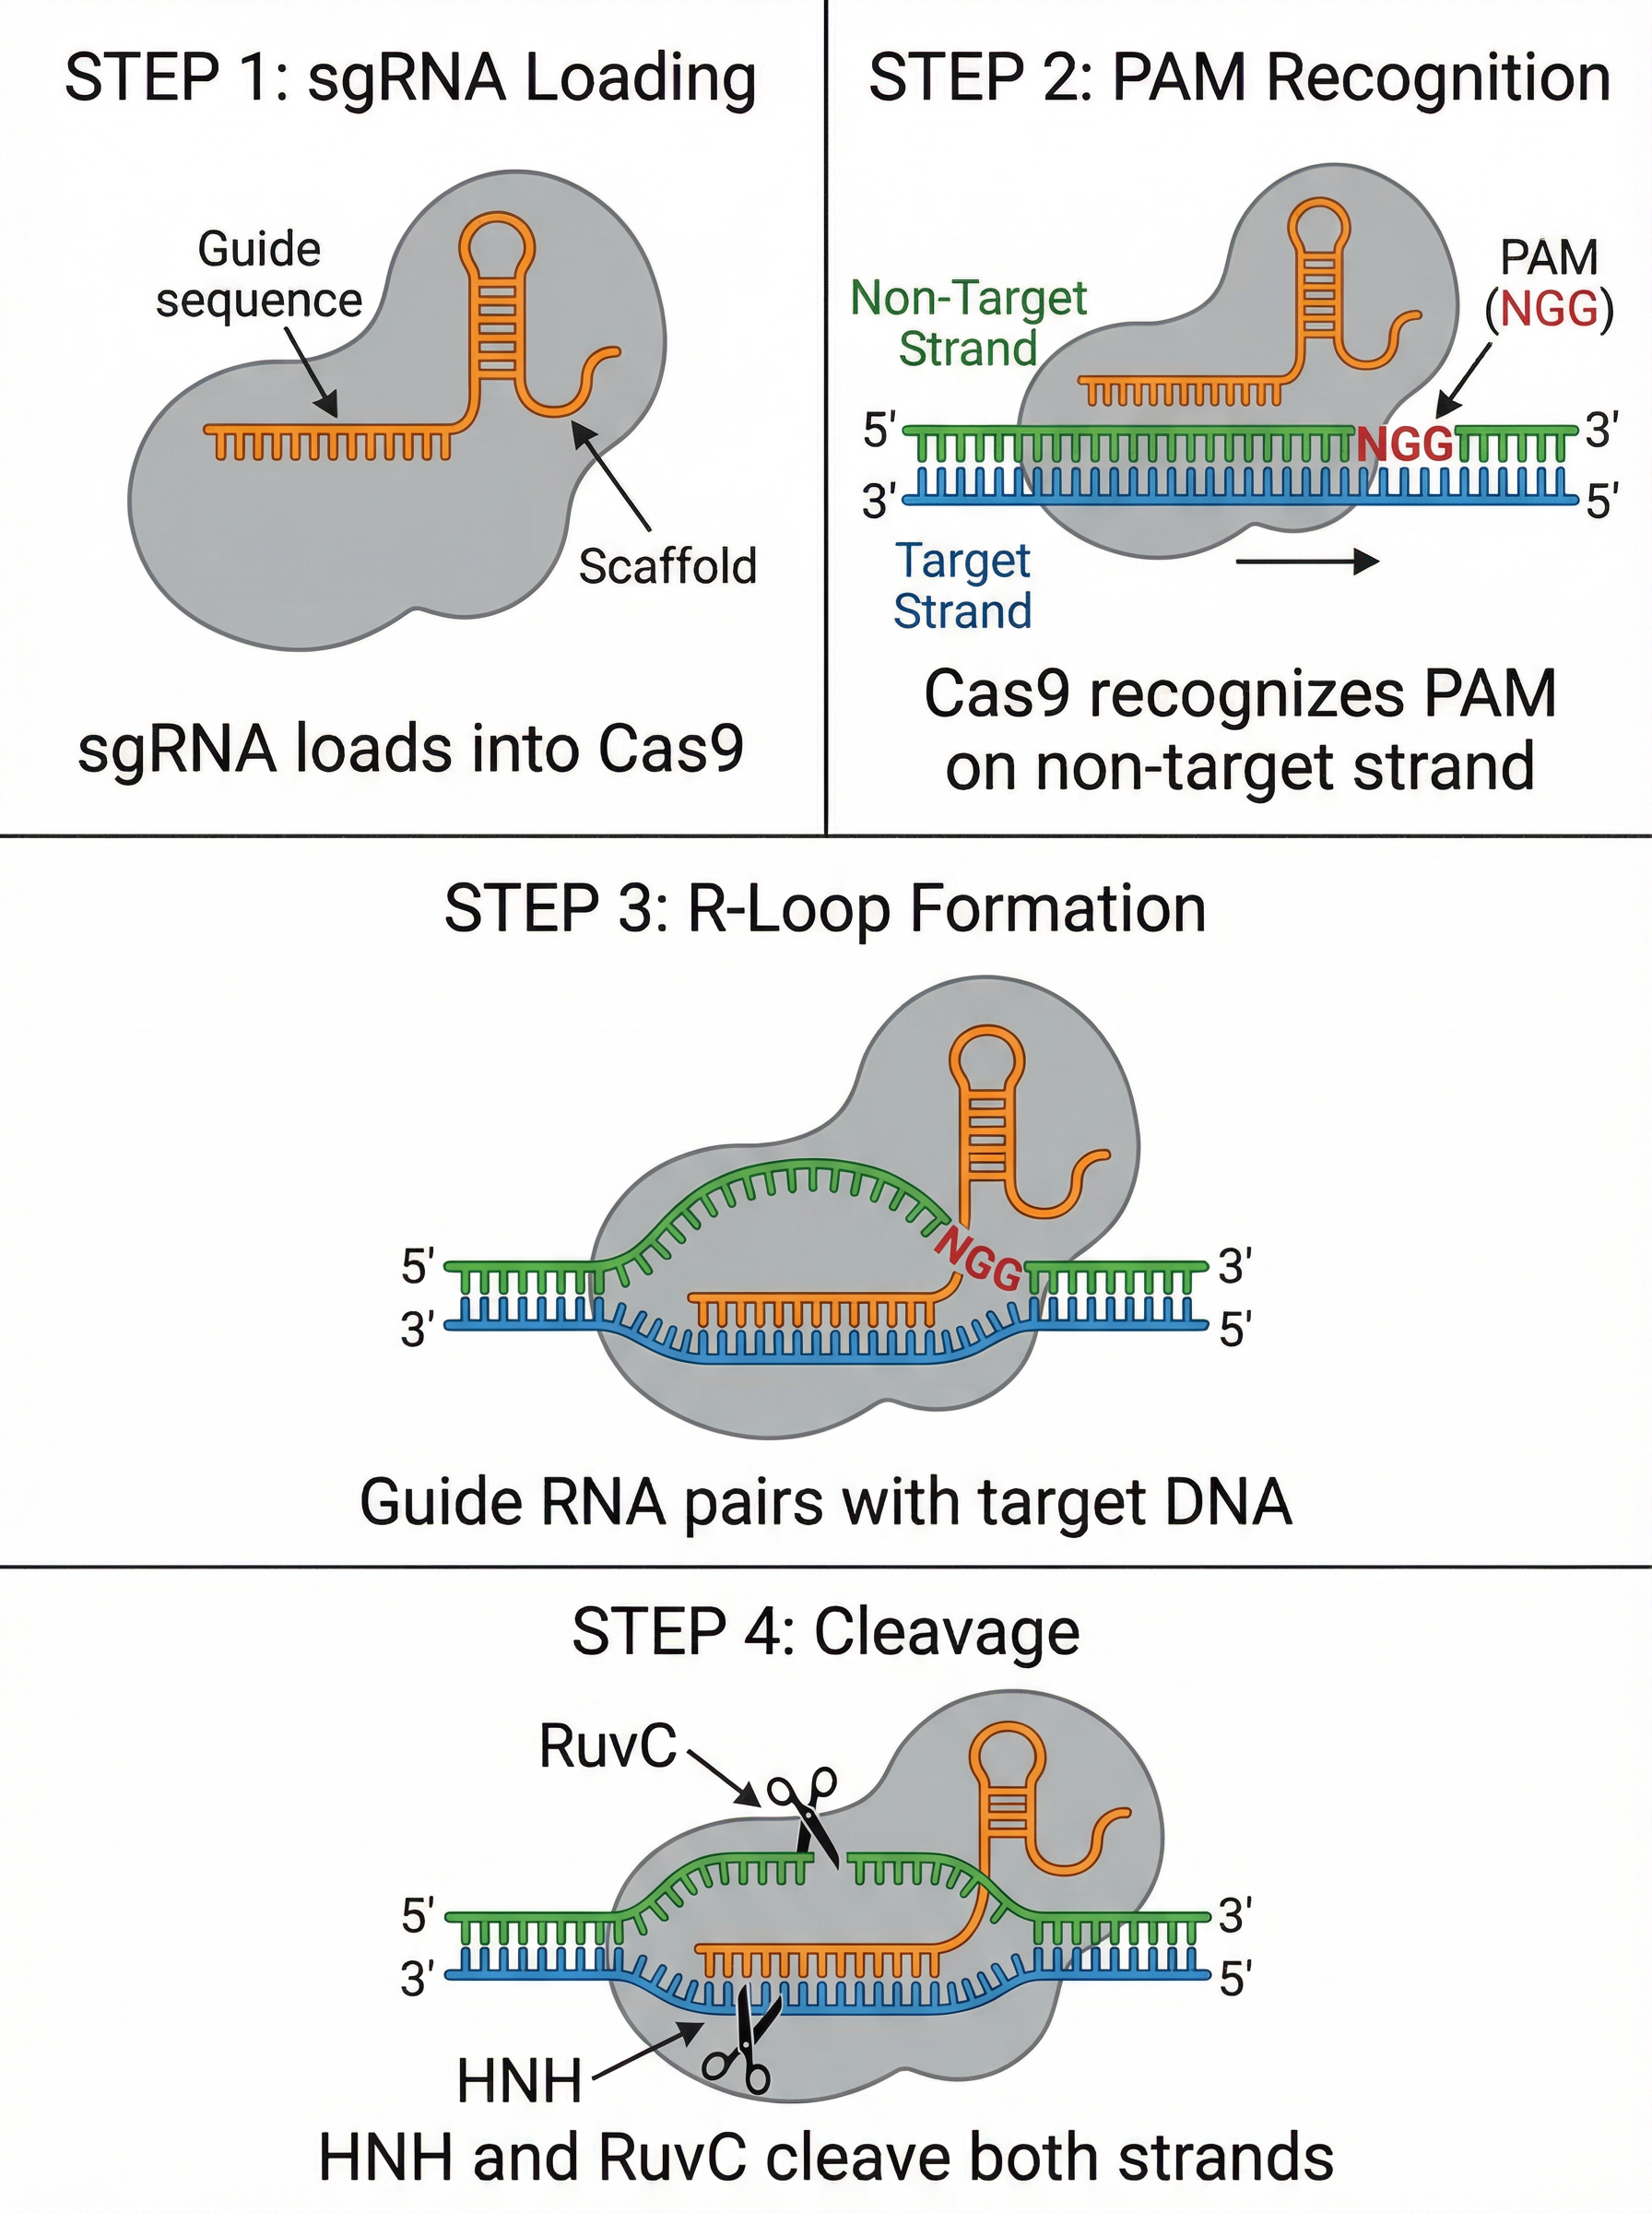
\includegraphics[width=0.9\textwidth]{Figs/CRISPR.png}
\caption{CRISPR-Cas9 mechanism showing the four-step process: (1) sgRNA loading into Cas9, (2) PAM recognition on the non-target strand, (3) R-loop formation as the guide RNA pairs with target DNA, and (4) double-strand cleavage by the HNH and RuvC nuclease domains.}
\label{fig:crispr-mechanism}
\end{figure}

Figure~\ref{fig:crispr-mechanism} illustrates the complete CRISPR-Cas9 editing mechanism, which proceeds through four sequential steps. Below, we define each key term shown in the figure to ensure accessibility for readers from diverse backgrounds:

\begin{description}
\item[sgRNA (single guide RNA):] A synthetic RNA molecule ($\sim$100 nucleotides) that combines two components: (i) a \textbf{guide sequence} (also called spacer; the corresponding target DNA sequence is termed the protospacer, $\sim$20 nucleotides) that determines target specificity by complementary base-pairing with the target DNA, and (ii) a \textbf{scaffold} region that forms secondary structures recognized by the Cas9 protein.

\item[Cas9:] The CRISPR-associated protein 9, a large ($\sim$1,400 amino acids) RNA-guided endonuclease that cleaves double-stranded DNA. The most commonly used variant is \textit{Streptococcus pyogenes} Cas9 (SpCas9).

\item[PAM (Protospacer Adjacent Motif):] A short DNA sequence (5'-NGG-3' for SpCas9, where N is any nucleotide) located immediately downstream of the target site on the non-target strand. PAM recognition is essential for Cas9 activation and is mediated by arginine residues (Arg1333, Arg1335) that contact the GG dinucleotide in the DNA major groove.

\item[Target strand vs.\ Non-target strand:] The \textbf{target strand} (also called the complementary strand) is the DNA strand that base-pairs with the guide RNA. The \textbf{non-target strand} (also called the non-complementary strand or PAM strand) contains the PAM sequence and is displaced during R-loop formation.

\item[R-loop:] A three-stranded nucleic acid structure formed when the guide RNA hybridizes with the target DNA strand, displacing the non-target strand. R-loop formation positions the DNA for cleavage by the Cas9 nuclease domains.

\item[HNH and RuvC domains:] The two nuclease domains within Cas9 responsible for DNA cleavage. The \textbf{HNH domain} cleaves the target strand (complementary to the guide), while the \textbf{RuvC domain} cleaves the non-target strand. Both cuts occur approximately 3 base pairs upstream of the PAM, generating a blunt-ended double-strand break (DSB).

\item[Double-strand break (DSB):] The DNA lesion created by Cas9 cleavage, which is subsequently repaired by cellular pathways: non-homologous end joining (NHEJ, error-prone, often causing insertions/deletions) or homology-directed repair (HDR, precise, requires a repair template).
\end{description}

SpCas9 editing requires a \(\sim 20\)-nt protospacer and a nearby \PAM{} (typically NGG), followed by \CasNine\ binding and cleavage~\citep{jinek2012,hsu2014}. Observed efficacy varies with:
\begin{itemize}
\item \textbf{Sequence effects} (motifs/composition such as GC content).
\item \textbf{\gRNA\ structure/thermodynamics} that can influence guide availability.
\item \textbf{Chromatin accessibility/state} that modulates Cas9 access (e.g., nucleosome occupancy and accessibility)~\citep{horlbeck2016,isaac2016}.
\end{itemize}

\section{On-target predictors: what is typically modeled}

Most on-target predictors map a sequence representation (one-hot, engineered features, or pretrained embeddings) through a learned backbone (CNN/RNN/attention) to output an efficacy score. Representative baselines include DeepHF~\citep{wang2019}, DeepSpCas9~\citep{kim2019deepspcas9}, and ChromeCRISPR~\citep{daneshpajouh2025chromecrispr}. Context-aware models incorporate chromatin accessibility or related epigenomic signals when available, such as CRISPRon~\citep{xiang2021}.

\paragraph{Very recent (2025) on-target models (verified for this thesis scope).}
To keep this proposal concise while reflecting the latest literature, we highlight five 2025 models that motivate the ChromaGuide design space:
\begin{itemize}
\item \textbf{CRISPR\_\allowbreak HNN} (Li et al., 2025): a hybrid MSC +\allowbreak multi-head self-attention (MHSA) +\allowbreak BiGRU model for on-target activity prediction~\citep{li2025crisprhnn}.
\item \textbf{PLM-CRISPR} (Hou et al., 2025): cross-variant prediction that represents Cas9 variants using ESM2 protein language model embeddings~\citep{hou2025plmcrispr}.
\item \textbf{CRISPR-FMC} (Li et al., 2025): a dual-branch architecture for on-target prediction that fuses one-hot sequence features with pretrained RNA embeddings via cross-branch interactions~\citep{li2025crisprfmc}.
\item \textbf{Graph-CRISPR} (Jiang et al., 2025): a graph neural network model that integrates sequence and \sgRNA\ secondary structure features for on-target efficiency prediction~\citep{jiang2025graph-crispr}.
\item \textbf{ChromeCRISPR} (Daneshpajouh et al., 2025): a CNN+RNN (CNN--GRU) hybrid baseline for on-target prediction, emphasizing strong sequence modeling with lightweight auxiliary features (e.g., GC content)~\citep{daneshpajouh2025chromecrispr}.
\end{itemize}

\paragraph{Why protocol choice matters.}
Reported headline metrics remain sensitive to dataset choice and leakage/split design; realistic evaluation therefore requires gene-held-out and cross-domain (dataset/cell-line) stress tests.

% Table omitted for concision (models discussed in text).

\section{Off-target effects and prediction methods}

Off-target activity arises when a \gRNA\ partially matches additional genomic loci that are adjacent to a compatible \PAM{} and permissive to Cas9 binding and cleavage. Key determinants include (i) mismatch number and position (with the PAM-proximal ``seed'' typically less tolerant), (ii) mismatch type and local sequence context, (iii) DNA/RNA bulges, and (iv) chromatin accessibility and other epigenomic factors that can modulate cleavage probability at both intended and unintended loci.

\paragraph{Experimental profiling of off-targets.}
Genome-wide assays such as GUIDE-seq provide empirical off-target site lists and approximate relative activities, and are commonly used to benchmark computational predictors and guide model training/evaluation~\citep{tsai2015guideseq}.

\paragraph{Four families of computational methods.}
Off-target prediction methods can be grouped into:
\begin{enumerate}
\item \textbf{Alignment-based:} enumerate candidate off-target loci by genome-wide approximate matching under PAM and mismatch/bulge constraints (e.g., Cas-OFFinder)~\citep{bae2014casoffinder}.
\item \textbf{Formula-based:} compute mismatch-position-weighted scores (e.g., MIT score, CFD score) and aggregate them into guide-level specificity estimates (often used in pipelines such as CRISPOR)~\citep{doench2016,haeussler2016}.
\item \textbf{Energy-based:} approximate Cas9--\gRNA--DNA binding/cleavage energetics to score the likelihood of cleavage (e.g., CRISPRoff~\citep{alkan2018crispr}).
\item \textbf{Deep learning / foundation models:} learn site-level cleavage probabilities directly from \sgRNA\--target pairs, optionally integrating epigenomic context (e.g., DeepCRISPR, CCLMoff, DNABERT-Epi)~\citep{chuai2018,du2025cclmoff,kimata2025dnabertepi}.
\end{enumerate}

\paragraph{Recent SOTA: CCLMoff (Du et al., 2025).}
Du et al. introduced \textbf{CCLMoff}, a transformer-based off-target predictor that incorporates a pretrained RNA language model and reports AUROC $=0.996$ in a cross-dataset evaluation setting (train on CIRCLE-seq, test on GUIDE-seq), outperforming a range of prior deep learning baselines~\citep{du2025cclmoff}.

\paragraph{Epigenomics-aware foundation model: DNABERT-Epi (Kimata \& Satou, 2025).}
Kimata and Satou introduced \textbf{DNABERT-Epi}, which fine-tunes a DNABERT foundation model and integrates epigenetic features (H3K4me3, H3K27ac, and ATAC-seq). They benchmark against five baselines across seven off-target datasets and report competitive or superior performance, highlighting the value of combining sequence pretraining with local chromatin context for off-target risk prediction~\citep{kimata2025dnabertepi}.

\paragraph{Broader chromatin-aware landscape.}
Beyond DNABERT-Epi, several other studies have explored integrating chromatin context into \sgRNA\ efficacy prediction. CRISPRscan~\citep{moreno2015crisprscan} was among the first to observe that local chromatin accessibility correlates with on-target cleavage, though it relied on hand-crafted sequence features rather than learned representations. More recently, \textbf{CRISPR-ML}~\citep{xiang2021crisprml} showed that appending DNase-seq and histone-mark signals to sequence embeddings yields statistically significant gains on held-out cell lines, albeit with a conventional gradient-boosted-tree architecture. \textbf{EpiCRISPR}~\citep{zhang2023epicrispr} adopted a multi-task neural network that jointly predicts on-target efficiency and chromatin state, demonstrating improved generalization when transferring across tissue types. Despite these advances, no existing method simultaneously addresses three challenges that ChromaGuide targets: (i)~learning chromatin representations end-to-end from raw epigenomic tracks rather than pre-computed summary features, (ii)~providing calibrated prediction intervals that remain reliable under distributional shift, and (iii)~evaluating under gene-held-out and dataset-held-out protocols that prevent data leakage.

\begin{table}[ht]
\centering
\caption{Quantitative comparison of representative off-target prediction methods. AUROC and PR-AUC are reported on GUIDE-seq evaluation sets where available. Epig. = epigenomic features used.}
\label{tab:offtarget-comparison}
\small
\begin{tabular}{llccc}
\hline
\textbf{Method} & \textbf{Category} & \textbf{AUROC} & \textbf{PR-AUC} & \textbf{Epig.} \\
\hline
CFD score~\citep{doench2016} & Formula & 0.925 & 0.066 & No \\
Cas-OFFinder~\citep{bae2014casoffinder} & Alignment & -- & -- & No \\
CRISPRoff~\citep{alkan2018crispr} & Energy & -- & -- & No \\
DeepCRISPR~\citep{chuai2018} & DL & -- & -- & Optional \\
CRISPR-Net~\citep{lin2020crisprnet} & DL & 0.993 & 0.292 & No \\
CCLMoff~\citep{du2025cclmoff} & DL + LM & 0.996 & -- & No \\
DNABERT-Epi~\citep{kimata2025dnabertepi} & DL + FM & -- & 0.550 & Yes \\
\hline
\end{tabular}
\end{table}

\section{\sgRNA\ design principles and tools}

Practical \sgRNA\ design aims to select guides with high on-target activity while controlling off-target risk, under hard constraints such as PAM availability and experiment-specific requirements (e.g., U6 promoter compatibility). This is commonly operationalized as (i) generating candidate guides at a locus, (ii) predicting on-target efficacy, (iii) screening/penalizing off-targets, and (iv) selecting a final guide under an explicit efficiency--specificity trade-off.

\paragraph{Taxonomy of on-target predictors.}
On-target efficiency models can be grouped into:
\begin{itemize}
\item \textbf{Conventional ML:} feature-engineered models such as Azimuth/Rule Set 2~\citep{doench2016}.
\item \textbf{Deep learning / pretrained models:} sequence models that learn representations directly from data, sometimes augmented with thermodynamic/structural/epigenomic signals or pretrained embeddings (e.g., CRISPRon, DeepHF, DeepSpCas9, CRISPR\_HNN, CRISPR-FMC, Graph-CRISPR, PLM-CRISPR)~\citep{xiang2021,wang2019,kim2019deepspcas9,li2025crisprhnn,li2025crisprfmc,jiang2025graph-crispr,hou2025plmcrispr}.
\end{itemize}

\begin{sloppypar}
\paragraph{Anchor models and benchmarks.}
Classic deep learning baselines remain widely used: CRISPRon~\citep{xiang2021}, DeepHF~\citep{wang2019}, and DeepSpCas9~\citep{kim2019deepspcas9}. A benchmark and ensemble study by Chen and Wang (Bioinformatics 2022) compared 17 published scoring algorithms across 16 datasets totaling $>90{,}000$ gRNAs and identifies CRISPRon, DeepSpCas9, and DeepHF as top-performing individual predictors, with ensemble approaches (e.g., sgDesigner and TSAM) also ranking strongly~\citep{chen2022ensemble}.
\end{sloppypar}

\paragraph{Very recent 2025 trends.}
Recent SOTA work emphasizes (i) hybrid local+global architectures with dynamic feature weighting (CRISPR\_HNN)~\citep{li2025crisprhnn}, (ii) pretrained embeddings and cross-modal fusion (CRISPR-FMC; Graph-CRISPR)~\citep{li2025crisprfmc,jiang2025graph-crispr}, and (iii) cross-variant generalization by integrating Cas9 variant representations from protein language models (PLM-CRISPR)~\citep{hou2025plmcrispr}. \textbf{ChromaGuide} is explicitly designed to synthesize all three dominant 2024--2025 trends: (i) it inherits the hybrid CNN-RNN backbone from ChromeCRISPR that parallels the local+global strategy of CRISPR\_HNN; (ii) its multi-modal fusion of sequence embeddings with epigenomic tracks aligns with the cross-modal paradigm of CRISPR-FMC and DNABERT-Epi; and (iii) its gene-held-out and cross-dataset evaluation protocol directly tests the generalization challenge that PLM-CRISPR addresses via protein language models. No existing method combines all three.

\paragraph{Design tools.}
End-to-end design tools implement candidate enumeration and integrate on-target and off-target scoring (e.g., CRISPOR, CHOPCHOP), often with practical filters and batch scoring capabilities~\citep{haeussler2016,labun2016chopchop}.

\section{Summary: method capabilities and gap analysis}
\label{sec:gap-analysis}

Table~\ref{tab:method-comparison} maps representative methods to the capabilities most relevant to this proposal. The three gaps that \textbf{ChromaGuide} targets---cell-specific epigenomic integration, calibrated uncertainty, and shift-aware evaluation---are not jointly addressed by any existing method.

\begin{table}[htbp]
\centering
\caption{Comparison of representative \sgRNA\ prediction methods across key capabilities. Columns indicate whether a method incorporates epigenomic context (Epi.), provides calibrated uncertainty estimates (Unc.), includes an off-target module (OT), and has been evaluated under gene-held-out or cross-dataset splits (Shift).}
\label{tab:method-comparison}
\small
\begin{tabular}{lcccc}
\hline
\textbf{Method} & \textbf{Epi.} & \textbf{Unc.} & \textbf{OT} & \textbf{Shift} \\
\hline
DeepCRISPR~\citep{chuai2018} & \checkmark$^\dagger$ & & & \\
CRISPRon~\citep{xiang2021} & & & & \checkmark \\ DeepHF~\citep{wang2019} & & & & \\ CCLMoff~\citep{du2025cclmoff} & & & \checkmark & \checkmark \\
CRISPR\_HNN~\citep{li2025crisprhnn} & & & & \\
PLM-CRISPR~\citep{hou2025plmcrispr} & & & & \\
CRISPR-FMC~\citep{li2025crisprfmc} & & & & \\
Graph-CRISPR~\citep{jiang2025graph-crispr} & & & \checkmark & \\
DNABERT-Epi~\citep{kimata2025dnabertepi} & \checkmark & & \checkmark & \\
Cas-OFFinder~\citep{bae2014casoffinder} & & & \checkmark & \\
CRISPOR~\citep{haeussler2016} & & & \checkmark & \\
ChromeCRISPR~\citep{daneshpajouh2025chromecrispr} & & & & \\
\hline
\textbf{ChromaGuide} & \checkmark & \checkmark & \checkmark & \checkmark \\
\hline
\end{tabular}
\vspace{2pt}\par\noindent{\footnotesize $^\dagger$Uses optional pre-computed epigenomic features rather than end-to-end learned chromatin representations from raw tracks.}
\end{table}

\paragraph{Research group context.}
The Wiese Computational Biology Laboratory at SFU brings over 25 years of experience in computational biology and bioinformatics, with foundational contributions spanning evolutionary algorithms for RNA secondary structure prediction, machine learning for biological sequence analysis, and, most recently, deep learning for CRISPR guide design~\citep{daneshpajouh2023navitas,daneshpajouh2023comparison,daneshpajouh2025chromecrispr}. This sustained research program---from early Canadian AI conference papers (2004) to the present---provides both the domain expertise and the benchmarking infrastructure upon which ChromaGuide is built. The progression from systematic model comparison~\citep{daneshpajouh2023comparison} to the ChromeCRISPR hybrid architecture~\citep{daneshpajouh2025chromecrispr} and now to the multi-modal ChromaGuide framework reflects a deliberate, incremental research strategy that mitigates technical risk.
